% Layout: (_4,(_3,_2)):(_1,(_4,_12))
\documentclass[convert]{standalone}
\usepackage{tikz}

\begin{document}
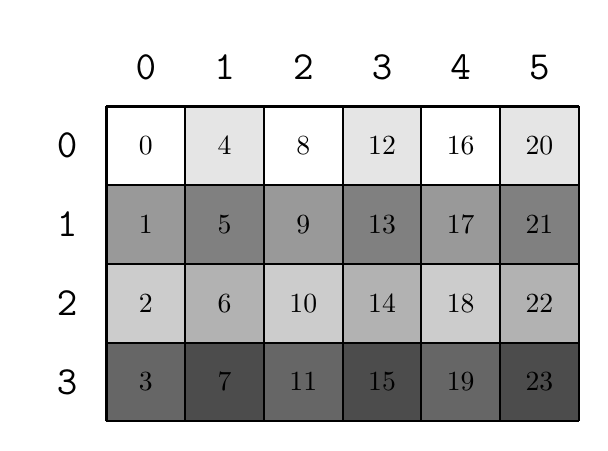
\begin{tikzpicture}[x={(0cm,-1cm)},y={(1cm,0cm)},every node/.style={minimum size=1cm, outer sep=0pt}]

\node[fill=black!00] at (0,0) {0};
\node[fill=black!10] at (0,1) {4};
\node[fill=black!00] at (0,2) {8};
\node[fill=black!10] at (0,3) {12};
\node[fill=black!00] at (0,4) {16};
\node[fill=black!10] at (0,5) {20};
\node[fill=black!40] at (1,0) {1};
\node[fill=black!50] at (1,1) {5};
\node[fill=black!40] at (1,2) {9};
\node[fill=black!50] at (1,3) {13};
\node[fill=black!40] at (1,4) {17};
\node[fill=black!50] at (1,5) {21};
\node[fill=black!20] at (2,0) {2};
\node[fill=black!30] at (2,1) {6};
\node[fill=black!20] at (2,2) {10};
\node[fill=black!30] at (2,3) {14};
\node[fill=black!20] at (2,4) {18};
\node[fill=black!30] at (2,5) {22};
\node[fill=black!60] at (3,0) {3};
\node[fill=black!70] at (3,1) {7};
\node[fill=black!60] at (3,2) {11};
\node[fill=black!70] at (3,3) {15};
\node[fill=black!60] at (3,4) {19};
\node[fill=black!70] at (3,5) {23};
\draw[color=black,thick,shift={(-0.5,-0.5)}] (0,0) grid (4,6);

\node at (0,-1) {\Large{\texttt{0}}};
\node at (1,-1) {\Large{\texttt{1}}};
\node at (2,-1) {\Large{\texttt{2}}};
\node at (3,-1) {\Large{\texttt{3}}};
\node at (-1,0) {\Large{\texttt{0}}};
\node at (-1,1) {\Large{\texttt{1}}};
\node at (-1,2) {\Large{\texttt{2}}};
\node at (-1,3) {\Large{\texttt{3}}};
\node at (-1,4) {\Large{\texttt{4}}};
\node at (-1,5) {\Large{\texttt{5}}};
\end{tikzpicture}
\end{document}
